\section{Optimisation of {BNN}s using different  inputs}\label{sec:GA:ResultDiffAN}

%\subsection{Parameter space sensitivity of cost functions}

%\subsection{Performance of best genomes and cross-comparison of cost functions}


% \section{Results}

% \subsection{Target Network}

\subsection{Genetic Algorithm Performance}


\subsubsection{Evolution of Cost Functions}

The performance of the {\GA} optimization is illustrated by the evolution of the
best score in each generation for three independent {\GA} runs
(Figure~\ref{fig:GA:R1}). The best genome score in each generation (solid line)
shows the progress of the optimization by the {\GA}, from large steps initially to
more incremental improvements as the score tends towards an asymptote.  During
the later generations the best genome score showed relatively little variability
between different {\GA} runs, suggesting that {\GA} performance was consistent across
runs. The relative improvement between initial and final scores was greater for
the ST and AIV cost functions than for the IFR cost function.
% {\GA} runs using both the ST and IFR cost functions attained final scores that
% were essentially identical to the target score (mark on right), but {\GA} runs
% using the AIV cost function attained final scores that did not reach the
% target score.

\begin{figure}[t!]
  \centering
  % \figfont{A}\hspace{3.2in}\figfont{B}\\
  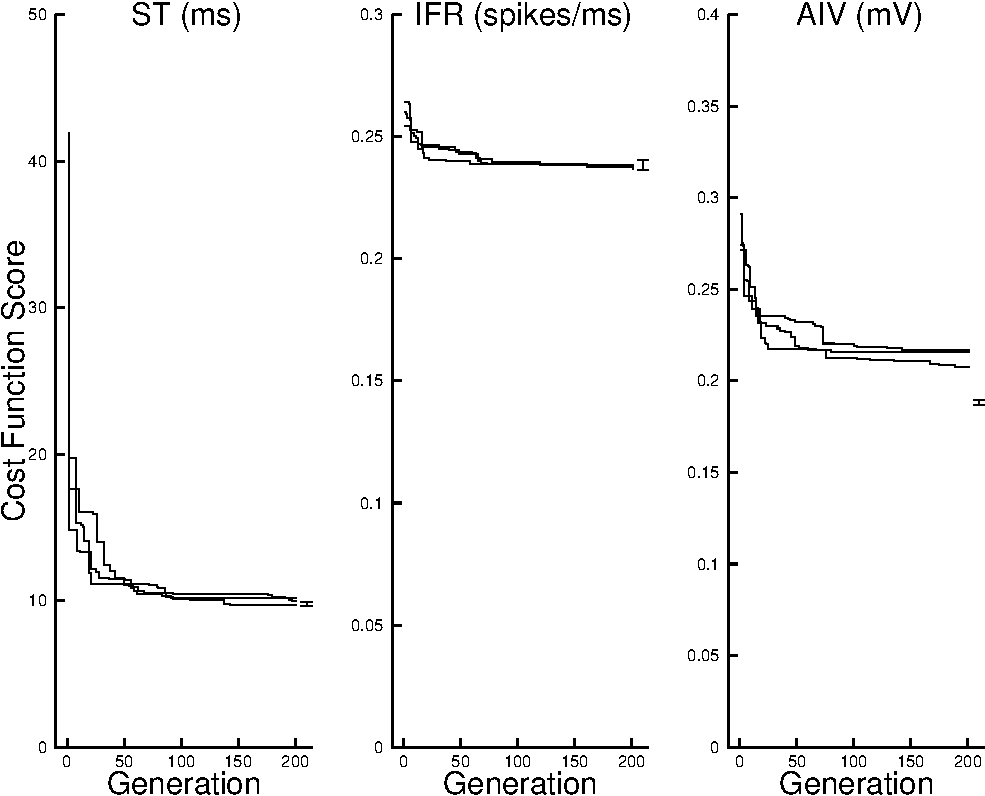
\includegraphics[width=\textwidth]{All25GAPerf-Stretch.eps}
  \caption[Performance of the {GA}]{Performance of the {GA}s best performing genome in each
    generation is shown for each simulation. The mark to the right of
    each graph is the mean score and 95 percentile range of the target
    genome (error bars 2*sd).}\label{fig:GA:R1}
\end{figure}

\smallskip{}

For all three cost functions the best score obtained by the {\GA} was considerably
above an error of zero. This does not imply poor performance by the {\GA}, because
a perfect score of zero would require not only an exact match to the target
parameters, but also a precise match to the auditory nerve input spike trains
used in the target data. Experimentally the spike times of the auditory nerve
vary stochastically based on an instantaneous rate function for any given
stimulus. This stochasticity was incorporated into our model and led to non-zero
scores, even for the target network. The mean target score is shown by the error
bars on the right of each plot in Figure~\ref{fig:GA:R1}.

\smallskip{}

For the ST and IFR cost functions the best genome score was within the range of
scores found for the target network, indicating that the {\GA} was able to find a
network that gave the same behaviour as the target network, as measured by the
cost function. For the AIV cost function, the best genome had a score that was
greater that the range of scores found for the target network, indicating a
discrepancy between the behaviour of the best network and that of the target, as
measured by the cost function.




\subsubsection{Cost Function Cross Comparison}

To facilitate the comparison of cost function performance, we used the best
genome from {\GA} runs trained with one of the cost functions to evaluate the
remaining cost functions. This also allowed us to gauge how well that genome was
able to generalize to reproduce network behaviour as measured by the other cost
functions.


\begin{figure}[th!]
  \centering
%  \includegraphics[width=\textwidth]{boxplot25-sep-st.eps}\\
%  \includegraphics[width=\textwidth]{boxplot25-sep-ifr.eps}\\
%  \includegraphics[width=\textwidth]{boxplot25-sep-iv.eps}\\
  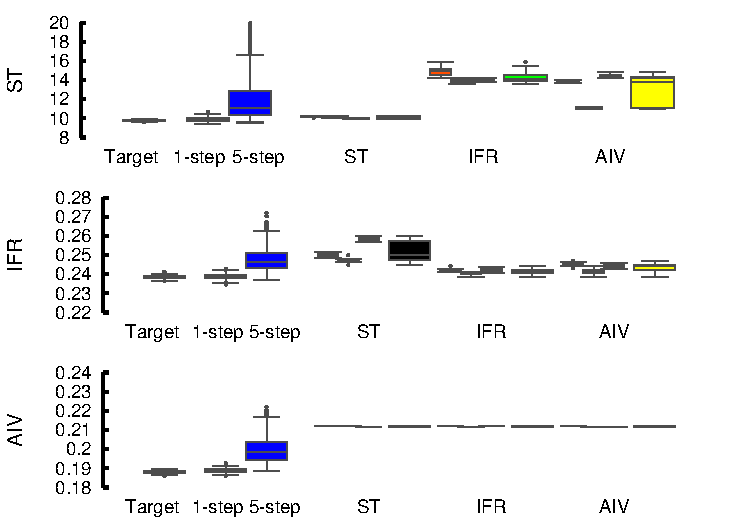
\includegraphics[width=\textwidth]{boxplot25-sep.eps}\\
  \caption[Cross comparison of best genomes]{Cross comparison of best genomes generated using {GA} with 25
    repetitions, measured against the target, 1-step and 5-step
    parameter perturbation distributions.  The boxplots show the all
    three best genomes evaluated ten times for each cost function,
    plus an accumulation boxplot of all three. 100 evaluations of the
    target genomes were evaluated and 1000 parameter perturbations
    were evaluated for the 1-step and 5-step
    distributions.}\label{fig:GA:R2A}
\end{figure}

\smallskip{}

The results are shown in Figure~\ref{fig:GA:R2A}, which compares the mean
score evaluated using the ST, IFR and AIV cost functions (top to
bottom, respectively) for each of the three best genomes obtained from
{\GA} runs trained with the different cost functions. In general, the
lowest scores were obtained when using the same cost function for
evaluation as was used for training of the best genome.

\smallskip{}

One AIV trained best genome generated ST scores around the target distribution,
however, the top graph shows that overall the IFR and AIV best genomes performed
relatively poorly when evaluated against the ST cost function.  The opposite
pattern was observed when the best genomes were evaluated with the IFR cost
function (middle plot), in which the ST best genomes performed poorly relative
to the IFR and AIV best genomes. All the best genomes gave similar scores for
the AIV cost function (bottom plot), but did not reach the target genome scores.

% the the ST trained genomes generalized
% well, in that the scores they obtained evaluating with the IFR and AIV cost
% function were close to the minimum score obtained across all genomes (i.e. the
% score obtained using the same cost function for the evaluation and training). In
% contrast, IFR and AIV trained genomes obtained relatively poor ST cost function
% scores compared with minimum score. They were, however, able to obtain near
% minimal scores with each other's cost function (i.e. the IFR trained genomes
% evaluated with the AIV cost function and vice versa).

% These results indicate that, in the current situation, training the {\GA} using
% spike timing information gave a better general match to data than using
% repetition-averaged information involving spike rate or intracellular voltage.


% The results are given in
% Table~\ref{tab:Best25}, which lists the mean and standard deviation of cost
% function scores from evaluations with 100 stochastically different AN
% inputs. When evaluated with either the ST or the AIV cost functions, the best
% genome with the lowest score was the one trained using the cost function
% itself (indicated by a ``*" in each column); i.e. the ST trained genome gave
% lowest ST score and the AIV trained genome gave the lowest AIV score, amongst
% the different genomes. However when evaluated using the IFR cost function, the
% best genome trained with this cost function performed worse than the other two
% best genomes. Networks trained with ST and AIV cost functions generalized well
% when network behaviour was measured using the other two cost functions,
% whereas the network trained with the IFR cost function generalized relatively
% poorly.


% \begin{tabularx}{0.95\textwidth}{Xcc}
%   Simulation                & MeanPE  & Score   \\\hline
%   stdyn diffAN sim1 min ga  & 22.1167 & 	10.1671 \\ 
%   stdyn diffAN sim2 min ga  & 31.6833 & 	10.0115 \\ 
%   stdyn diffAN sim3 min ga  & 12.7833 & 	9.67888 \\ \hline 
%   ifrga25 diffAN sim1 min ga& 22.2833 & 	0.238577 \\ 
%   ifrga25 diffAN sim2 min ga& 25.3167 & 	0.236389 \\ 
%   ifrga25 diffAN sim3 min ga& 28.5167 & 	0.23757 \\ \hline
%   ivga25 diffAN sim1 min ga & 26.2833 & 	0.216678 \\ 
%   ivga25 diffAN sim2 min ga &  25.45  & 0.207727 \\ 
%   ivga25 diffAN sim3 min ga & 29.3833 & 	0.21564 \\\hline
% \end{tabularx}

\clearpage



\subsubsection{Match to Target Parameters}

A further way to evaluate {\GA} performance is to compare the parameter values
between the best and target genomes by evaluating the relative error
between parameters (i.e. (target value - best value)/target value). Individual 
relative parameter errors are shown in Figure~\ref{fig:GA:R2} for
each of the best genomes trained on a particular cost function. Parameters
were ordered by increasing mean relative error across all genomes.

\smallskip{}

\begin{figure}[th!]
  \centering
  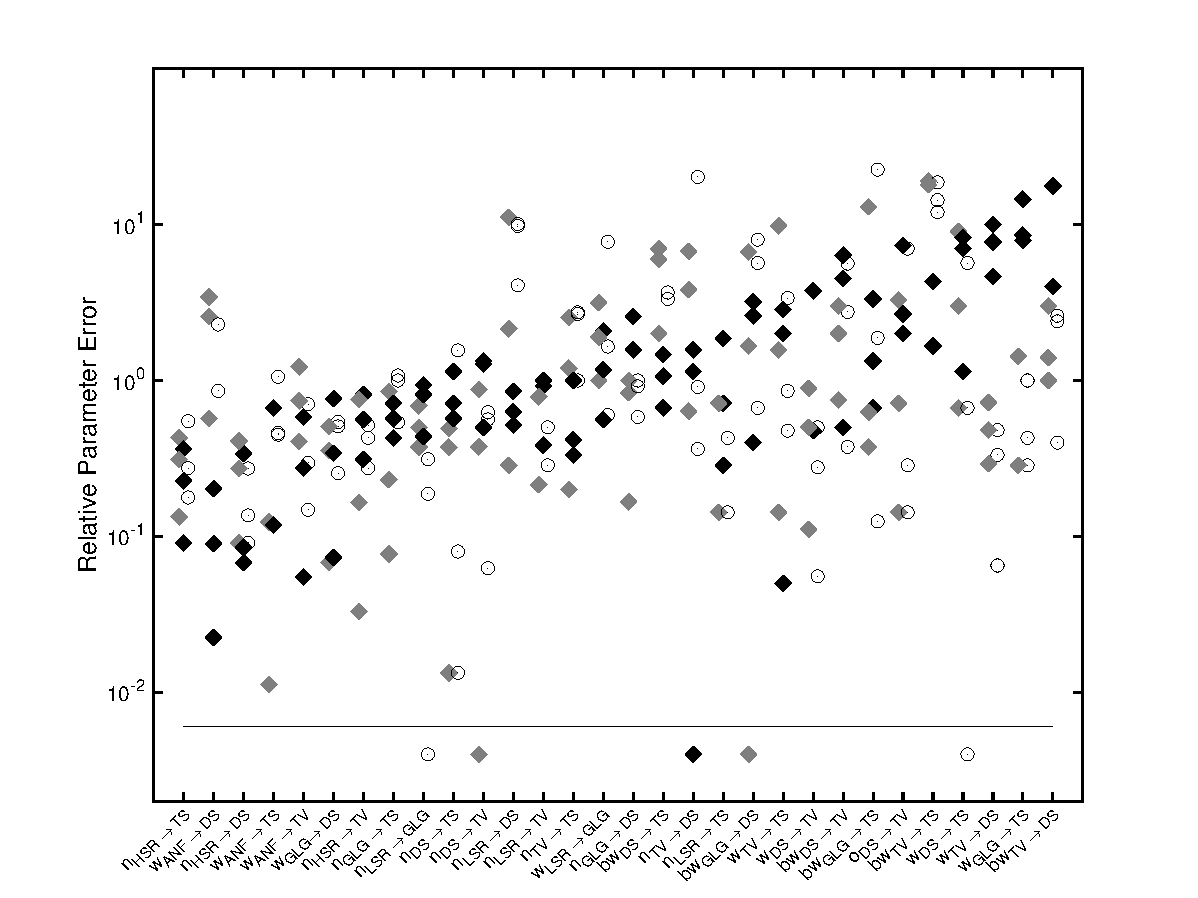
\includegraphics[width=\textwidth]{BestGenomesReRaw_CombinedLog}
  \caption[Best genome parameter errors]{Parameter errors of the best genomes in 3 {GA}
    simulations for each cost function: ST (grey diamond),%${\color{halfgray} \diamond}$), 
IFR (block diamond),%${\color{black} \diamond }$), 
and AIV (${\circ}$). Errors were normalised in terms
    of the target parameter values ( (target - bestgenome) / target )}\label{fig:GA:R2}
\end{figure}


The plot shows a similar level and pattern of performance across
genomes trained with the three different cost functions. Parameters were
either reasonably or poorly constrained independent of the cost function
being used in training.

\smallskip{}

In terms of parameter type, all bandwidth parameters were in the upper half
of genome errors whereas synapse number parameters were predominantly in
the lower half.  Weight parameters are spread over the whole range.


% {\it Still concerned that units are wrong. Percent error? Also v.hard compare
% cost functions. Plot on same figure? Looks like {\GA} run variability is so large
% that nothing can be said about best cost function.}  The error has been
% measured in terms of the unit steps that were used to discretize the
% parameter. This is an arbitrary scale that relies on the designer of the {\GA}
% choose a ``sensible" discretization scale for the parameters that
% 
% The lowest mean normalized parameter error was obtained by the AIV-trained
% best genome (0.207), followed by the ST-trained best genome (0.252) and the
% IFR-trained best genome (0.273). This order is consistent with performance of
% the different cost functions as evaluated by their cost function scores.

% In summary, the ST and AIV cost functions appear to perform better than the
% IFR cost function for {\GA} optimization. This conclusion is supported by
% comparison of best genome scores relative to target scores, cost function
% cross comparisons and analysis of parameter errors.
%% Rearange order and comment on similarity.


% When the inputs were randomized and the training data (25~reps)
% remained the same, the {\GA} populations' learning was considerably
% slower and the search space was more compact, Figure 6B. This meant
% that there was less difference between a good genome and a bad
% genome.  The best genome obtained by the IFR-25 cost function with
% different inputs had a score of 0.263~sp/ms and a mean parameter
% error of 0.273 (Figure~\ref{fig:GA:8}D).
% 
% The performance of the best genome generated by the AIV-25
% cost function with different inputs was very accurate for inhibitory
% parameters (Figure~\ref{fig:GA:8}G) presumably due to subthreshold
% information within the intracellular voltages.

\subsection{Parameter Sensitivity}\label{sec:GA:param-sens-results}

% Estimate of best performance possible given noisy input.
% 
% Comparison of ST, IFR and AIV.
% 
% Sensitivity - 1 step and 5-step.
% 
% Roughly equal sensitivity across cost functions.
% 
% The {\GA} run using the ST cost
% function and different {\ANF} inputs (Figure~\ref{fig:GA:5}B) had a similar
% learning profile, but there was less variability in the 25--75
% percentile range in the later generations and the best genome score
% was 9.72~ms (Figure~\ref{fig:GA:5}B).
% 
% 
% 
% When the inputs were
% randomized and the training data (25~reps) remained the same, the {\GA}
% populations' learning was considerably slower and the search space was
% more compact, Figure 6B. This meant that there was less difference
% between a good genome and a bad genome.  The best genome obtained by
% the IFR-25 cost function with different inputs had a score of
% 0.263~sp/ms and a mean parameter error of 0.273
% (Figure~\ref{fig:GA:8}D).
% 
% The AIV-25 and
% AIV-250 cost functions with different inputs scored, 0.208~and 0.188
% mV, respectively.  The mean parameter errors of the best genome for
% the AIV-25 cost function with identical inputs, the AIV-25 cost
% function with different inputs and the AIV-250 cost function with
% different inputs were, 0.258, 0.207 and 0.275, respectively (Figure
% 8F-H).

\subsubsection{Simultaneous Parameter Perturbation Analysis}\label{sec:GA:simult-param-pert}

To better understand the relationship between cost function scores and the match
to target parameter values a parameter sensitivity analysis was performed. This
involved measuring the change in the cost function due to simultaneous
perturbations in all parameters.  Figure~\ref{fig:GA:R3} shows the distribution of
cost function scores for different degrees of random simultaneous parameter
perturbation. Two populations of 1000 genomes were generated, one with parameter
values allowed to vary uniformly by 1 unit step either side of the target
(i.e. -1, 0 or 1 steps), and the second population was varied uniformly up to 5
unit steps.  In the 5 units step experiment, one parameter covers 11
combinations, including the target value.


\begin{figure}[th!]
  \centering
  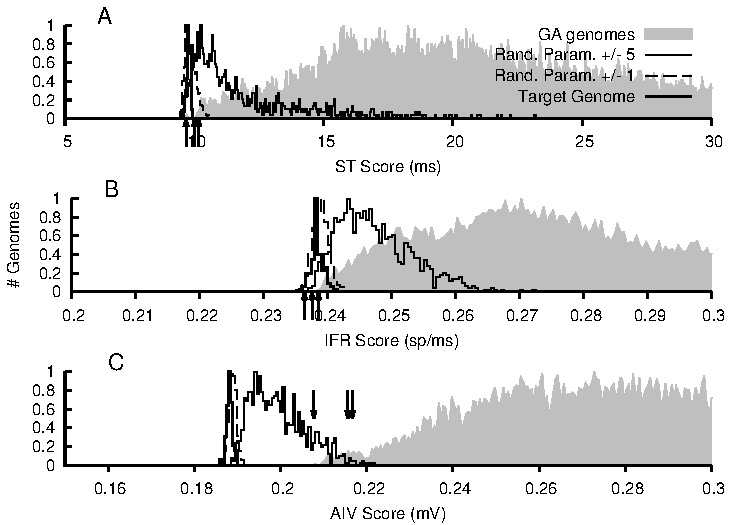
\includegraphics[width=\textwidth]{Histograms-Normalised.eps}  
  \caption[Histograms of parameter perturbations]{Histograms of simultaneous parameter perturbation of each cost
    function. The distribution of genomes in gray are all genomes evaluated by
    the {GA} that obtained the lowest score. The best scores of 3 {GA} simulations
    are pointed to by the arrows. The histograms show the distributions of 100
    target genome scores (thick line), 1000 genomes deviated by 1 unit step away
    from the target value (dashed line), and 1000 genomes deviated by 5 steps
    (thin line) from the target. The input spike generation and network
    connections for each parameter set (genome) were randomly generated for each
    evaluation.  All graphs are normalised to the peak value in each
    histogram.}\label{fig:GA:R3}
\end{figure}

% In total the 5 units step experiment covers 9.72\% of
% the total parameter space and the 1 unit step experiment covers
% 2.65\%. {\bf What does this mean?? 11\% relative error = 1 step on average}

\smallskip{}

In general, 1 unit step perturbations produced cost function scores both
slightly above and slightly below the range produced by the target network
(compare histograms in dashed versus bold lines, respectively). Five unit
step perturbations produced cost functions scores that were largely above
the target network range (compare histograms in thin solid versus bold
lines, respectively). This pattern was consistent across the three cost
function types. The shift of cost function scores to progressively higher
values with progressively larger perturbations is expected and
desirable. It forms the basis by which the {\GA} performs optimization by
comparing candidate genomes to the target.

% The distribution of cost functions scores for the 5 unit step perturbation is
% less highly sensitive cost function in the vicinity of the target parameter
% values. Separated from target distribution for the IFR cost function than for
% either of the other cost functions. This is consistent with generally poorer
% performance of the IFR cost function.

\smallskip{}

Best genomes scores from {\GA} runs trained with either the ST or the IFR cost
function lay inside the range produced by the 1 unit step perturbation, whereas
best genomes scores from the {\GA} runs trained with the AIV cost function were at
the upper limit of the range produced by 5 unit step perturbations. In fact,
Fig.~\ref{fig:GA:R2} shows that all best genomes scored equally badly when
evaluated 100 times with the AIV cost function. Given this difference in AIV
cost function scores, it is worth noting again that pattern of change in cost
function distributions with perturbation size was fairly consistent across cost
function types. This suggests that the AIV cost function is equally well behaved
in the vicinity of the target compared to the other two cost functions. In this
case, the reason the best genomes trained with any cost function were unable to
attain a score in the target range (bottom plot of Figure~\ref{fig:GA:R2}) was not
due to a poorly behaved cost function. \yellownote{but further explanation is unknown.}


\smallskip{}

It is, perhaps, surprising that the 1 unit step perturbations could produced a
network with lower cost function scores than the target network, albeit
marginally. This effect is the result of noise in the cost function, introduced
by the stochastic auditory nerve input: because the 1 unit step perturbations
involved 1000 separate instances of AN input, compared to only 100 instances for
the target, it was likely that a better match to the precise target AN input was
found amongst the former than the latter.  This effect is only expected to
become apparent for values of the cost function around the target score, where
systematic reduction of the cost function becomes increasingly marginal. This is
consistent with the observation that for larger, 5 unit step perturbations this
effect was much diminished or absent.


% When the target parameters were evaluated 100 times with different
% {\ANF} input spikes the distribution of the ST cost function scores
% moved to 9.72~ms ($\pm$ 0.06~ms) (Figure~\ref{fig:GA:9}B).  The 1-step
% distribution compressed around 9.79~ms for different inputs, As
% indicators of the {\GAs} final performance, the best genomes produced
% by the {\GA} of 8.45~ms (identical inputs) and 9.72~ms (different
% inputs) were very reasonable estimates.  The shape of the ST cost
% function distributions of 5 stp populations scores were very similar
% except for a positive shift with different inputs with means 10~ms
% and 11.8~ms, respectively.
% 
% Different {\ANF} inputs had an adverse effect on the learning
% performance of the IFR-25 cost function, with the {\GA} unable to find
% reasonable estimates near the global optimum
% (Figure~\ref{fig:GA:10}B). The 1 step and 5 step scores were
% distributed around or close to the target scores showing a
% compression of the global optimum around 0.25~sp/ms
% (Figure~\ref{fig:GA:10}B).
% 
% 
% Using different inputs, the target value of the AIV-25
% cost function is shifted to just above 0.2~mV, with the 1- and 5-step
% not far above. The best performing genomes in the {\GA} were very close
% to the range of the 1-step and target genome scores (inset
% Figure~\ref{fig:GA:11}B).




\subsection{Effects of Noise}\label{sec:GA:effects-noise}

Noise from auditory nerve inputs could have a significant impact on
the {\GA} optimization, with noise potentially preventing the {\GA} from
attaining a good match to target. A simple way to reduce noise is to
use a larger sample of stochastic realisations of the AN input when
evaluating target and candidate genomes. This can reduce noise through
an averaging process, in the case of IFR and AIV cost functions or
through allowing more choice in matching spike trains in the ST cost
function. This would require using more stimulus repetitions when
collecting target data experimentally, and when simulating candidate
networks in the {\GA} computationally. In this section we examine the
utility of this approach by comparing {\GA} performance for 100 versus 25
stochastically distinct repetitions of the AN input for both target
and candidate genomes.

\smallskip{}


\subsubsection{Increased Stimulus Presentations}

\begin{figure}[th!]
  \centering
  % \figfont{A}\hspace{3.2in}\figfont{B}\\
  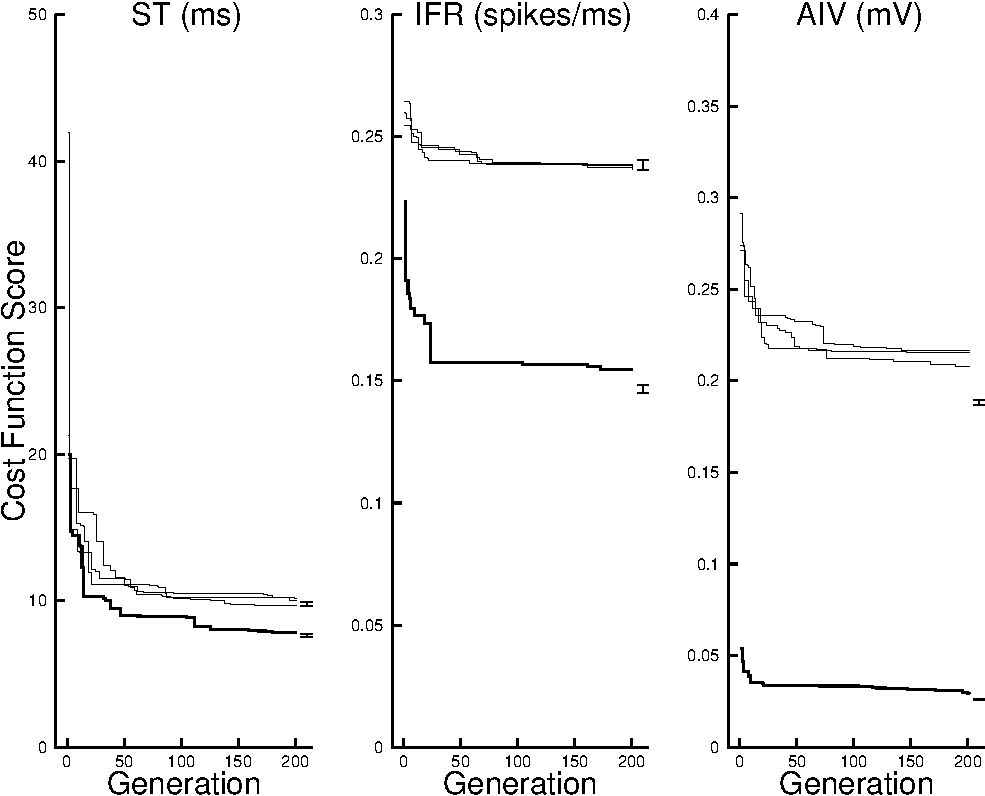
\includegraphics[width=\textwidth]{All100GAPerf-Stretch.eps}
  \caption[Performance of the {GA} (100 reps)]{Performance of the {GA}s best performing genome run with 100
    repetitions in the fitness function. {GA} simulations run with 25 repetitions are shown in grey. The mark to the right of each graph is the mean
    score and error bars showing the range of 2 times standard
    deviation away from the mean target genome score.}\label{fig:GA:R5}
\end{figure}

Figure~\ref{fig:GA:R5} shows the evolution of best genome scores when 100
repetitions were used for the target and candidate genomes instead of
25 (as used in the results presented thus far). Overall the use of
increased repetitions of the stimulus resulted in reduced cost
function scores but did not result in better {\GA} performance. This is
shown by the analysis given in Figure~\ref{fig:GA:R6}.

\smallskip{}

Similar to Fig~\ref{fig:GA:R2}A, the figure compares scores across best genomes
trained with different cost function types (ST, IFR or AIV) and different
numbers of repetition (25 or 100) giving a total of six different best genomes
types: ST25, ST100, IFR25, IFR100, AIV25 and AIV100. The three different graphs
(Fig~\ref{fig:GA:R2}A-C) correspond to evaluation of these best genomes using the
three different cost function types. The top of the lighter bars give the mean
score when 100 repetitions were used for evaluation, while the top of the
(appended) dark bars gives the mean score when only 25 repetitions were used
for evaluation.

\begin{figure}[th!]
  \centering
  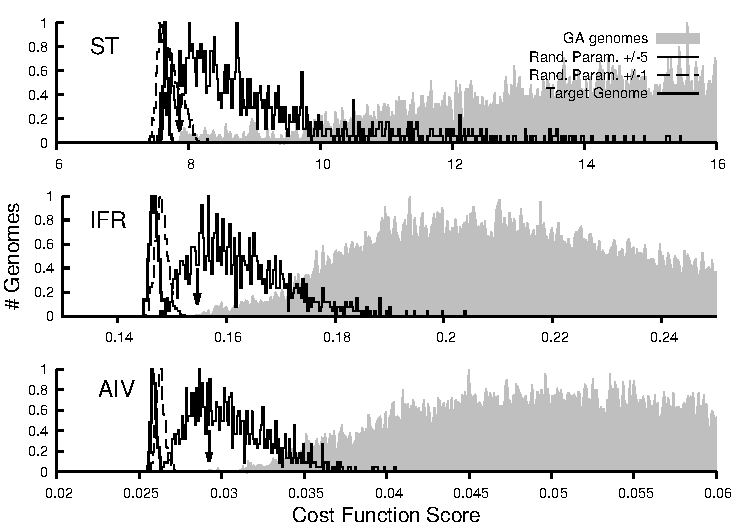
\includegraphics[width=\textwidth]{Histograms100-MaxNorm.eps}  
  \caption[Histograms of parameter perturbations (100 reps)]{Histograms of simultaneous parameter perturbation using 100
    repetitions. Similar to Fig.~\ref{fig:GA:R4}, the distribution of
    genomes evaluated during the {GA} are shown in gray and the eventual
    best score is pointed to by the arrow. The histograms show the
    distributions of 100 target genome scores (thick line), 1000
    genomes deviated by 1 unit step away from the target value (dashed
    line), and 1000 genomes deviated by 5 steps (thin line) from the
    target. The input spike generation and network connections for
    each parameter set (genome) were randomly generated for each
    evaluation.}
  \label{fig:GA:R6}
\end{figure}

\smallskip{}

In all cases the use of 100 repetitions to evaluate the cost function
resulted in lower scores than when 25 repetitions were used (i.e.\ the
top of the dark bar lies above the top of the light bar). This did not
imply that genomes trained with 100 repetitions attained lower scores
than those trained with 25 repetitions, once the comparison was made
using the same cost function (i.e.\ same type, same number of
repetitions). In nearly all cases, scores for genomes trained using
different numbers of repetition (25 or 100), but the same type of cost
function (ST, IFR or AIV), obtained similar scores, regardless of the
details of the cost function used to evaluate them (i.e. ST25, ST100,
IFR25, IFR100, AIV25 and AIV100 cost functions). The exception was the
AIV100 trained genome when evaluated by the ST cost
function. % check statistical difference of AIV in ST

\smallskip{}

This implies that, although the increased number of repetitions
reduced noise (and therefore cost function scores), this was not a
factor limiting {\GA} performance.

\begin{figure}[th!]
  \centering
  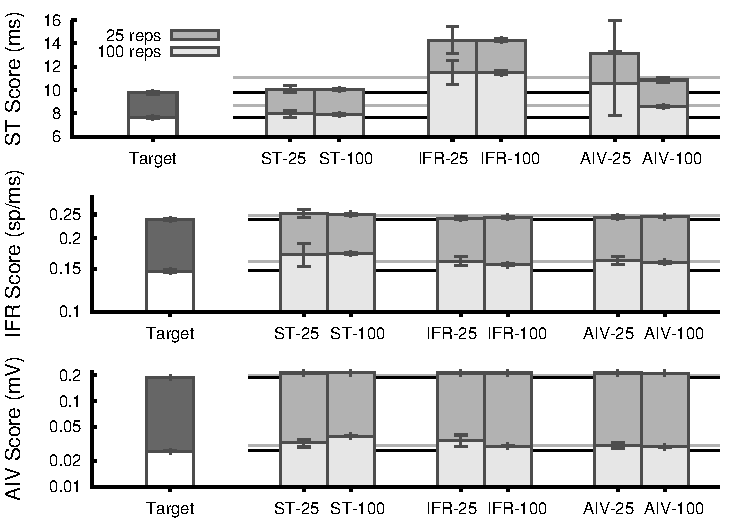
\includegraphics[width=\textwidth]{best25+100.eps}
  \caption[Comparison of best genomes]{Comparison of Best genomes trained with different inputs
    using 100 or 25 repetitions.  Target genome was run 100 times and
    each {GA} best genomes were run 10 times. For reference, horizontal
    lines show the the median of the distribution of parameter
    perturbation for 1-step (dark line) and 5-steps (light
    line).}\label{fig:GA:R7}
\end{figure}


\begin{table}[th]
  \centering
  \begin{tabularx}{0.95\textwidth}{Xccc}
Cost Function  & PE$^*$ & Final {\GA} Score & Mean (S.D)\\[0.5ex]\hline
   ST (ms)     & 1.977  &    7.86038     & 7.89 (0.04) \\
IFR (spikes/ms)& 2.169  &    0.154698    & 0.1557 (8.6E-4) \\
 AIV (mV/ms)   & 2.325  &   0.0292369    & 0.0292 (9.8E-5)\\ \hline
\end{tabularx}
  \caption{Best genomes obtained from {GA}s run with 100 repetitions. $*$ Mean relative parameter error. }
  \label{tab:BestGenome100}
\end{table}

\begin{figure}[th!]
  \centering
  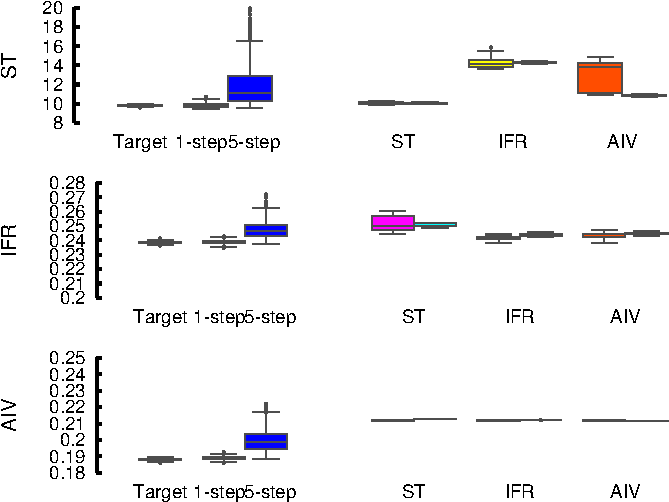
\includegraphics[width=\textwidth]{boxplot-100+25.eps}\\
  \caption{Cross comparison of best genomes generated using {GA} with
    100 repetitions, measured against the target, 1-step and 5-step
    parameter perturbation distributions.  The boxplots show the best
    genomes evaluated ten times for each cost
    function. }\label{fig:GA:BestGenome10025}
\end{figure}



% For comparison, also shown on these graphs are the best genome scores when
% only 25 repetitions were used, as well the accompanying histograms for the 1
% unit step perturbation analysis.
% 
% 
% {\it Perhaps present Figure showing target + best genome scores for ST, IFR
% and AIV trained as evaluated by each cost function} The 1 unit step
% perturbations scores for 100 repetitions are less than their counterparts for
% both 25 repetitions. This suggest that a substantial part of the cost function
% score, for 25 repetitions or ideal inputs, is attributable to noise. In the
% case of the ideal inputs, this noise is quenched in the form fixed random AN
% spike times and only becomes apparent when the number of synaptic connections
% in the network is perturbed from the target.
% 
%% Figure ? also shows that for the IFR cost function, the {\GA} was able to make
%% use of this reduced noise to obtain a best genome with a score close to the
%% target score, but for the AIV cost function, the {\GA} was not able to do
%% this. This is the reverse situation to when 25 repetitions were used for the
%% target.
% 
% Despite the reduction on cost function scores and noise did not help the {\GA}
% find better parameter fits: surprisingly parameter errors were worse than with
% 25 repetitions.
%% 
%% The individual parameter sensitivity analysis showed a very similar pattern to
% the case with 25 repetitions: similar sets of parameters showed either bilateral
% sensitivity, unilateral sensitivity, insensitivity or contained opposing
% gradients. By contrast, the pattern of sensitivity for ideal inputs was quite
% different. This suggest that the greater sensitivity exhibited in the case of
% ideal inputs was due to the effects of quenched noise in the AN inputs.
% 
% Table ? shows a cross comparison of cost function scores for best genomes
% trained with either 25 or 250 repetitions for the target. It indicates that
% training with a 250 repetition target did not result in better performing best
% genomes. The best genome trained with 25 repetitions performed comparably to
% or better than the best genome trained with 250 repetitions, whether its
% performance was evaluated using a cost function with 25 of 250 repetitions.
% 
% In summary, the analysis indicates that although increased repetitions lead to
% lower cost function scores for the best genomes attained by the {\GA}, these
% best genomes were no better those trained with 25 repetition in terms of
% parameter errors or cross comparison of cost function scores. The reduction in
% cost function score is simply due to a reduction in noise, but appears to
% provide no benefit for the {\GA} in terms of matching parameters to the target or
% reproducing the behaviour of the network.



% {\it Comment: There are two possible explanations for the increase in
% sensitivity when ideal input are used. The first is that the noise was masking
% an underlying trend or effect in the data, and that using ideal inputs
% eliminates this noises giving more sensitivity in the cost function to the
% underlying trend. The second is that the increased sensitivity for ideal input
% is a sensitivity to quenched noise in the input in the form of a specific set
% of spike times in the AN input. The former is a desirable property of the cost
% function, while the latter is not.
% 
% One way to differentiate between these possibilities is to increase the number
% of stimulus presentations. This can be used to reduce the noise by averaging
% and so better reveal the underlying effect. It is also a practical approach to
% overcoming the problem of input noise, since it can often be achieved
% experimentally.}



%%% Local Variables: 
%%% mode: latex
%%% TeX-master: "GAChapter"
%%% TeX-PDF-mode: nil
%%% End: 
